% Generated by `python -m experiments.experiment_2.appendix_captions` -- do not edit by hand.
% Main-text figure for Experiment 2. Needs \usepackage{graphicx}; paths are relative to outputs/finals/experiment-2/.
\begin{figure}[t]
  \centering
  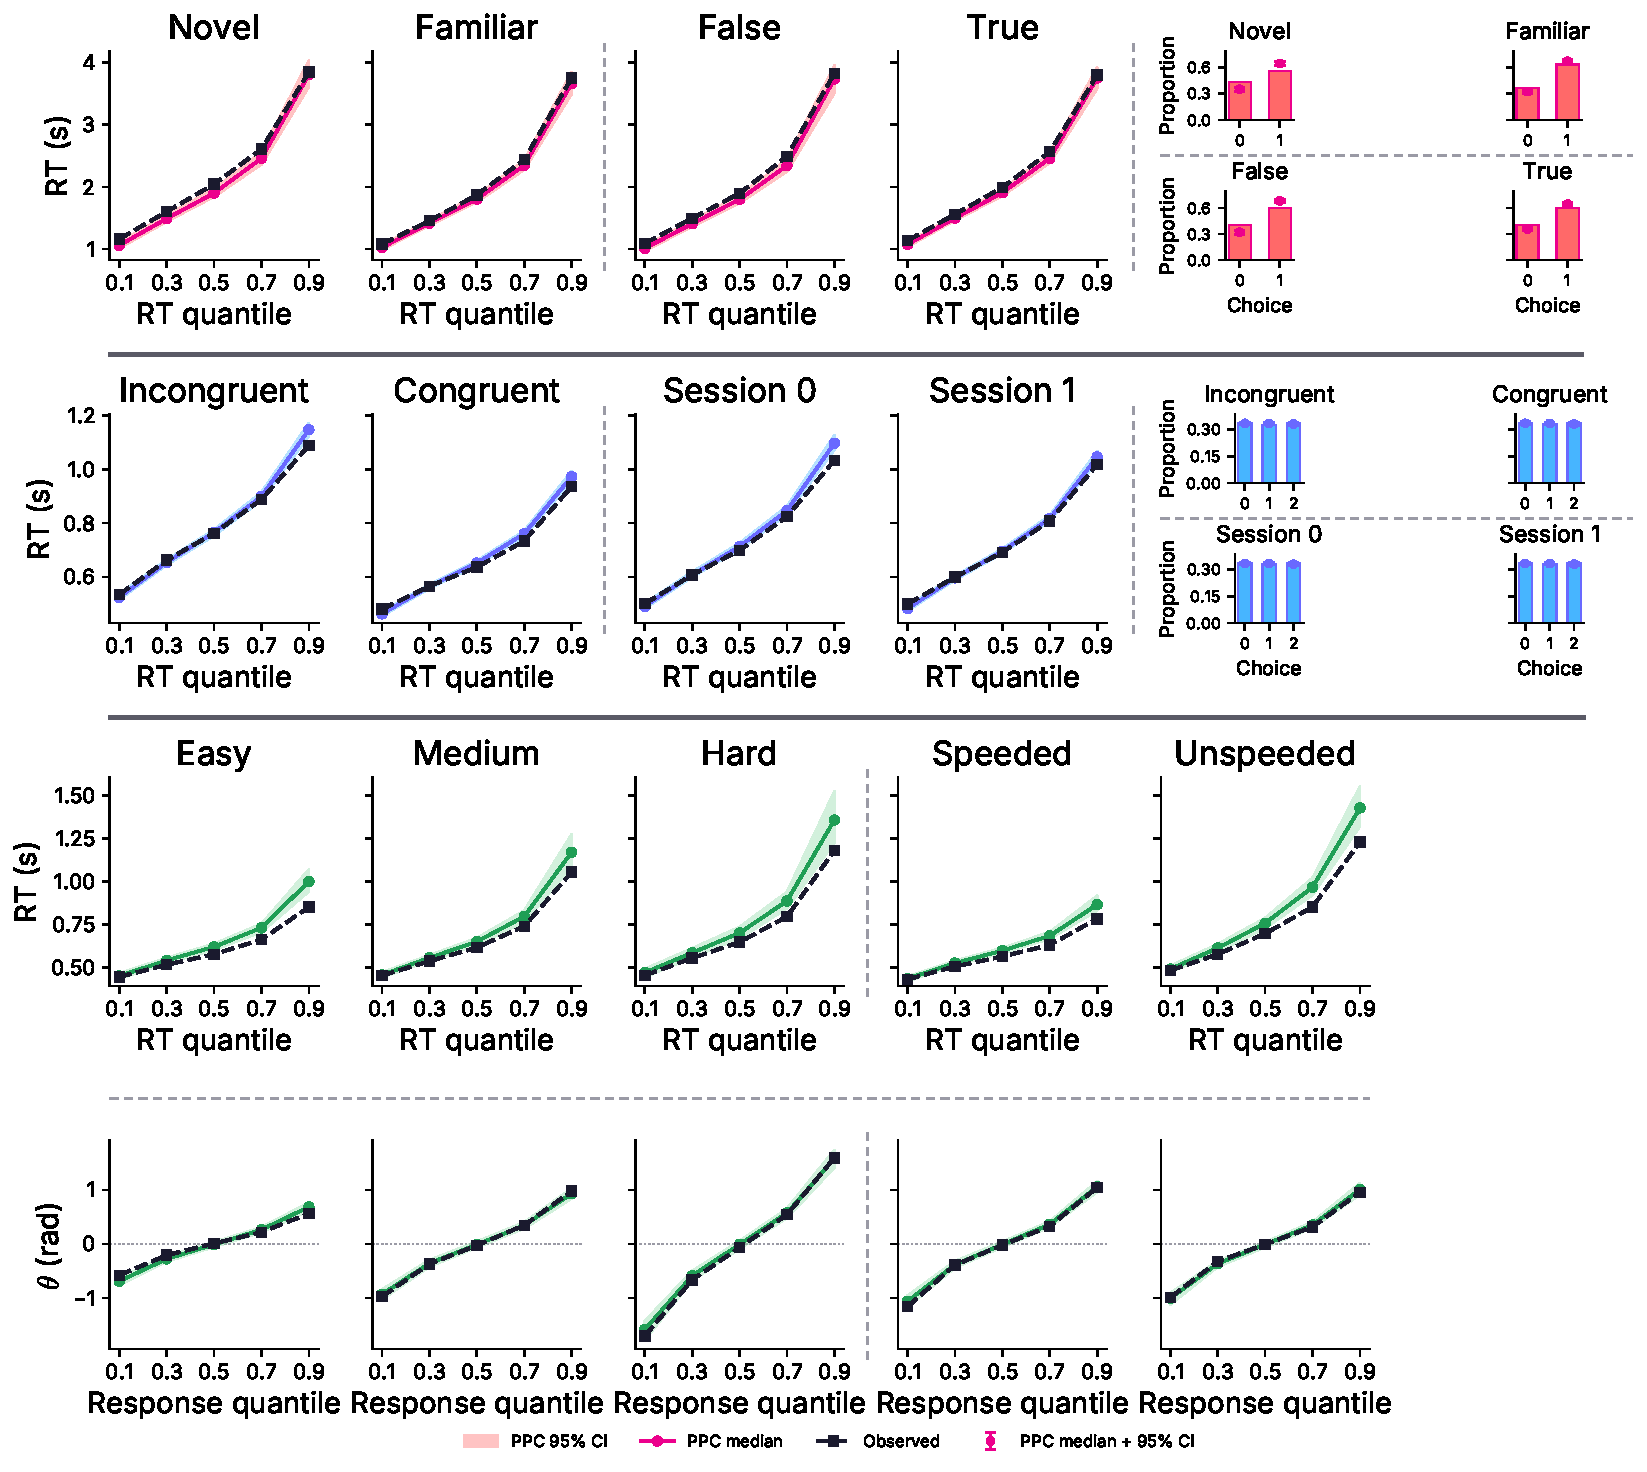
\includegraphics[width=\textwidth]{combined_ppc.pdf}
  \caption{\textbf{Posterior predictive checks on real data.} Observed data against the posterior predictive of CogFormer's fits, pooled over subjects: DDM (72 subjects; top row), RDM (149; second row) and CDM (12; bottom two rows). Quantile panels show the 0.1, 0.3, 0.5, 0.7 and 0.9 quantiles of RT (and, for the CDM, of the continuous response angle $\theta$, bottom row) for each level of each experimental condition: observed (black squares, dashed) against the predictive median (coloured line) with its 95\% interval (band). The $2 \times 2$ blocks on the right compare, per condition level, the observed proportion of each response (bars; DDM: the two responses, RDM: the three colour responses) with the predictive median and 95\% interval (points). Dashed rules separate conditions within a family, solid rules the families. Details in Appendix~\ref{app:exp2-main-details}.}
  \label{fig:exp2-main}
\end{figure}
